\documentclass[mathserif]{beamer}
\usetheme{Luebeck}
%\usepackage[francais]{babel}
\usepackage[utf8]{inputenc} % Uses the utf8 input encoding
\usepackage[T1]{fontenc} % Use 8-bit encoding that has 256 glyphs
\usepackage[style=authoryear,backend=biber]{biblatex}
\addbibresource{main.bib}

\usepackage[nomath]{kpfonts}
\usepackage{eulervm}
%\usepackage{default}

\usepackage{amsthm}
\usepackage{amssymb}
\usepackage{xparse}
\usepackage{thmtools}
\usepackage{stackrel}

%shortcuts
\newcommand{\R}{\mathbb{R}}
\newcommand{\C}{\mathbb{C}}
\newcommand{\Z}{\mathbb{Z}}
\newcommand{\N}{\mathbb{N}}
\newcommand{\fii}{\varphi}
\newcommand{\dd}{\mathrm{d}}
\newcommand{\CP}{\mathbb{CP}}
\renewcommand{\S}{\mathbb{S}}
\DeclareMathOperator{\Sp}{Sp}
\DeclareMathOperator{\tr}{tr}
\DeclareMathOperator{\dist}{dist}

% theorems configuration

\makeatletter
\newtheoremstyle{indented}
{7pt} %vertical space before
{7pt} % vertical space after
{} %{\addtolength{\@totalleftmargin}{2.5em}
	%\addtolength{\linewidth}{-3.5em}
	%\parshape 1 3.5em \linewidth} %body font
{1.5em} %indent
{\bfseries} %header font
{.} %punctuation
{.5em} %horizontal space after header
{} %header specification

\theoremstyle{definition}

\newtheorem{defn}{Définition}[section]

\theoremstyle{plain}
%\newtheorem*{theorem*}{Theorem}

\newtheorem{thm}{Théorème}

\renewcommand{\thetheorem}{\Alph{theorem}}
\newenvironment{preuve}{
	\noindent \textbf{Proof. }}{\hfill $\square$\medskip\par}

\newtheorem{exemple}[defn]{Example}
\newtheorem{prop}[defn]{Proposition}
\newtheorem{corr}[defn]{Corollary}
\newtheorem{por}[defn]{Porisme}
\newtheorem{ex}[defn]{Example}
\newtheorem{lem}[defn]{Lemma}
\newtheorem{conj}{Conjecture}
\newtheorem{ax}{Axiom}  %Axioms have their own numerotation

\theoremstyle{definition}
\newtheorem{rem}[defn]{Remark} %remarks are not indented
\newtheorem{rems}[defn]{Remarks}

%--------------
% Mise en page mathématique
%--------------
\addtolength{\jot}{.2em}


\title{Toeplitz
  operators and the large spin limit}
\author[Alix Deleporte]{Alix Deleporte\\Advisor : Nalini Anantharaman}
\institute[IRMA]{Institut de Recherche Mathématique
  Avancée\\Université de Strasbourg}
\titlegraphic{
\includegraphics[height=1cm]{ANR.png}}

\newcommand{\spline}{\hline}
\renewcommand{\arraystretch}{1.3}

\DeclareSourcemap{
  \maps[datatype=bibtex]{
    \map[overwrite=true]{
      \step[fieldsource=author,
            match=Deleporte,
            final]
      \step[fieldset=keywords, fieldvalue=Deleporte]
    }
  }
}
\begin{document}


\begin{frame}
	\titlepage
\end{frame}

\begin{frame}\frametitle{Introduction}
	\begin{itemize}
		\item Quantum spins: triplet of self-adjoint matrices
                  $(S_x,S_y,S_z)\in M_{2S+1}(\C)$,
                  with \[[S_x,S_y]=\frac{i}{S}S_z\] and similar
                  formulas given by direct permutation.
		\item $S=\frac 12$: Pauli matrices
		\[S_x=\tiny{\frac 12\begin{pmatrix}
		0& 1\\1& 0
		\end{pmatrix}}\quad S_y=\frac 12\begin{pmatrix}
		0& i\\-i& 0
		\end{pmatrix}\quad S_z=\frac 12\begin{pmatrix}
		1& 0\\0& -1
		\end{pmatrix}.\]
		\uncover<2>{\item Finite graph $G$ $\rightsquigarrow$ operator on $(\C^{2S+1})^{\otimes |G|}$:
		\[H_{AF}=\sum_{e\sim f}S_{x,e}S_{x,f}+S_{y,e}S_{y,f}+S_{z,e}S_{z,f}\]}
	\end{itemize}
      \end{frame}

            \begin{frame}
        \frametitle{Introduction}
%\begin{overlayarea}{\textwidth}{\textheight}
  \begin{center}
    \begin{picture}(50,50)
          \only<1>{\put(-100,-70){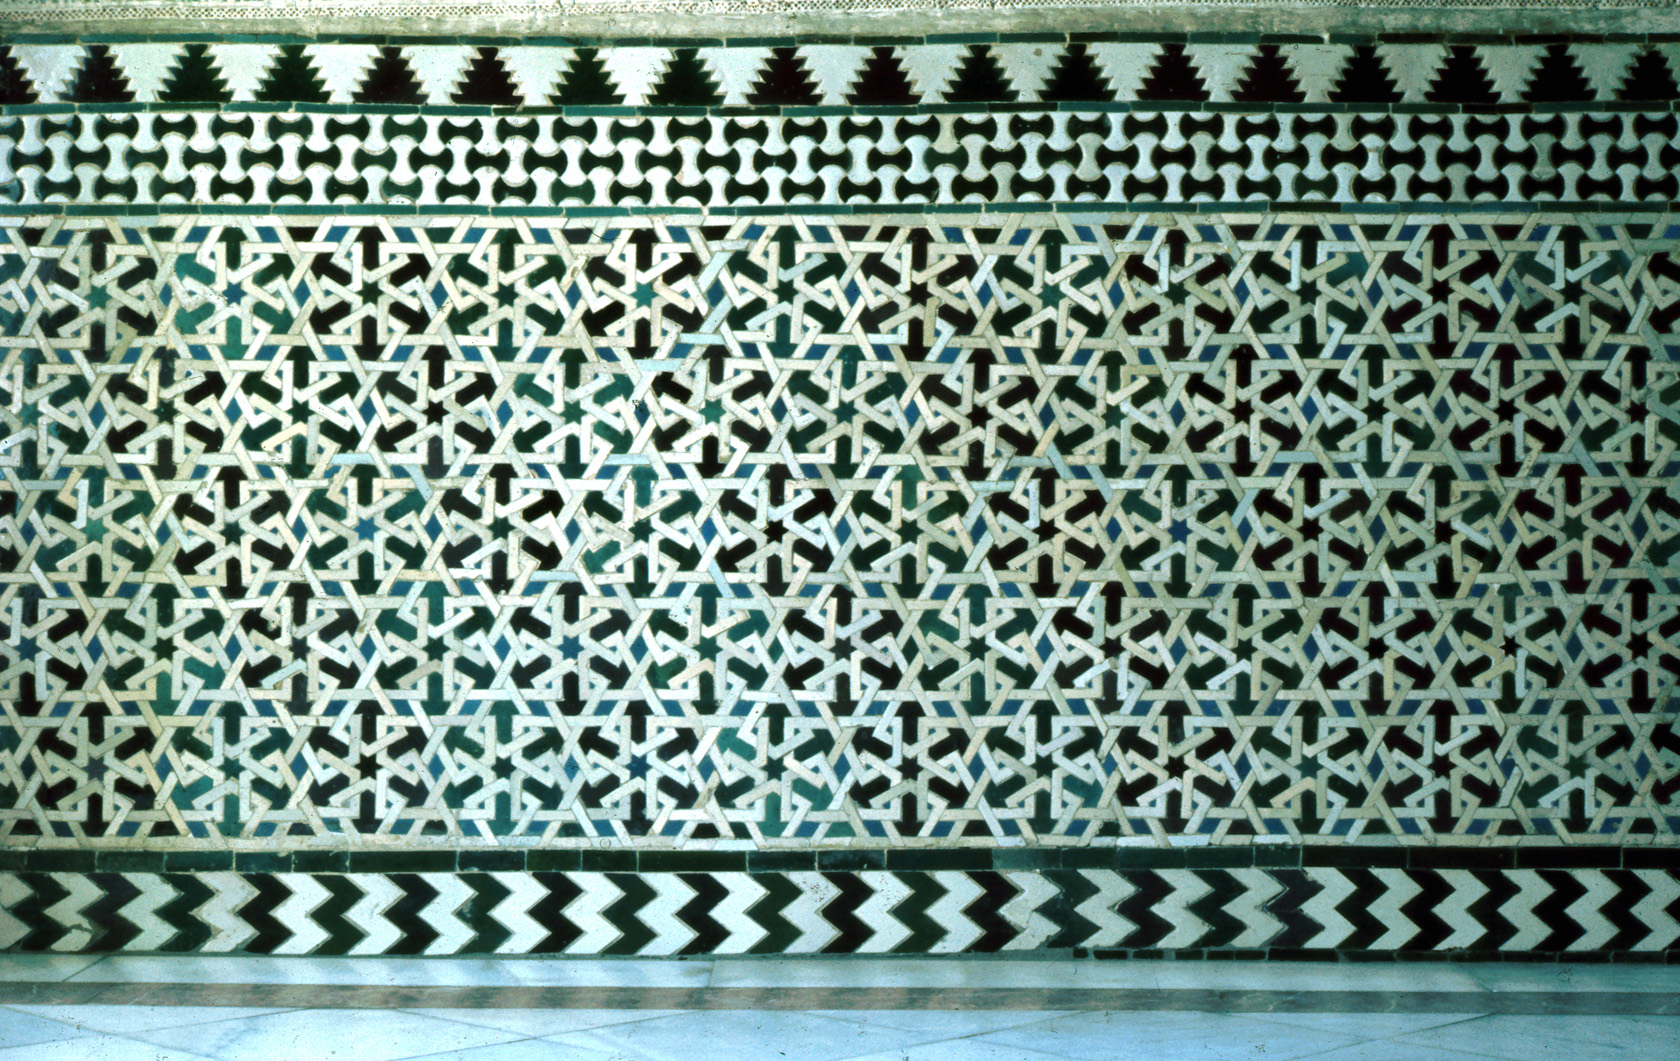
\includegraphics[scale=8]{Alcazar.png}}}
          \only<2>{\put(-100,-70){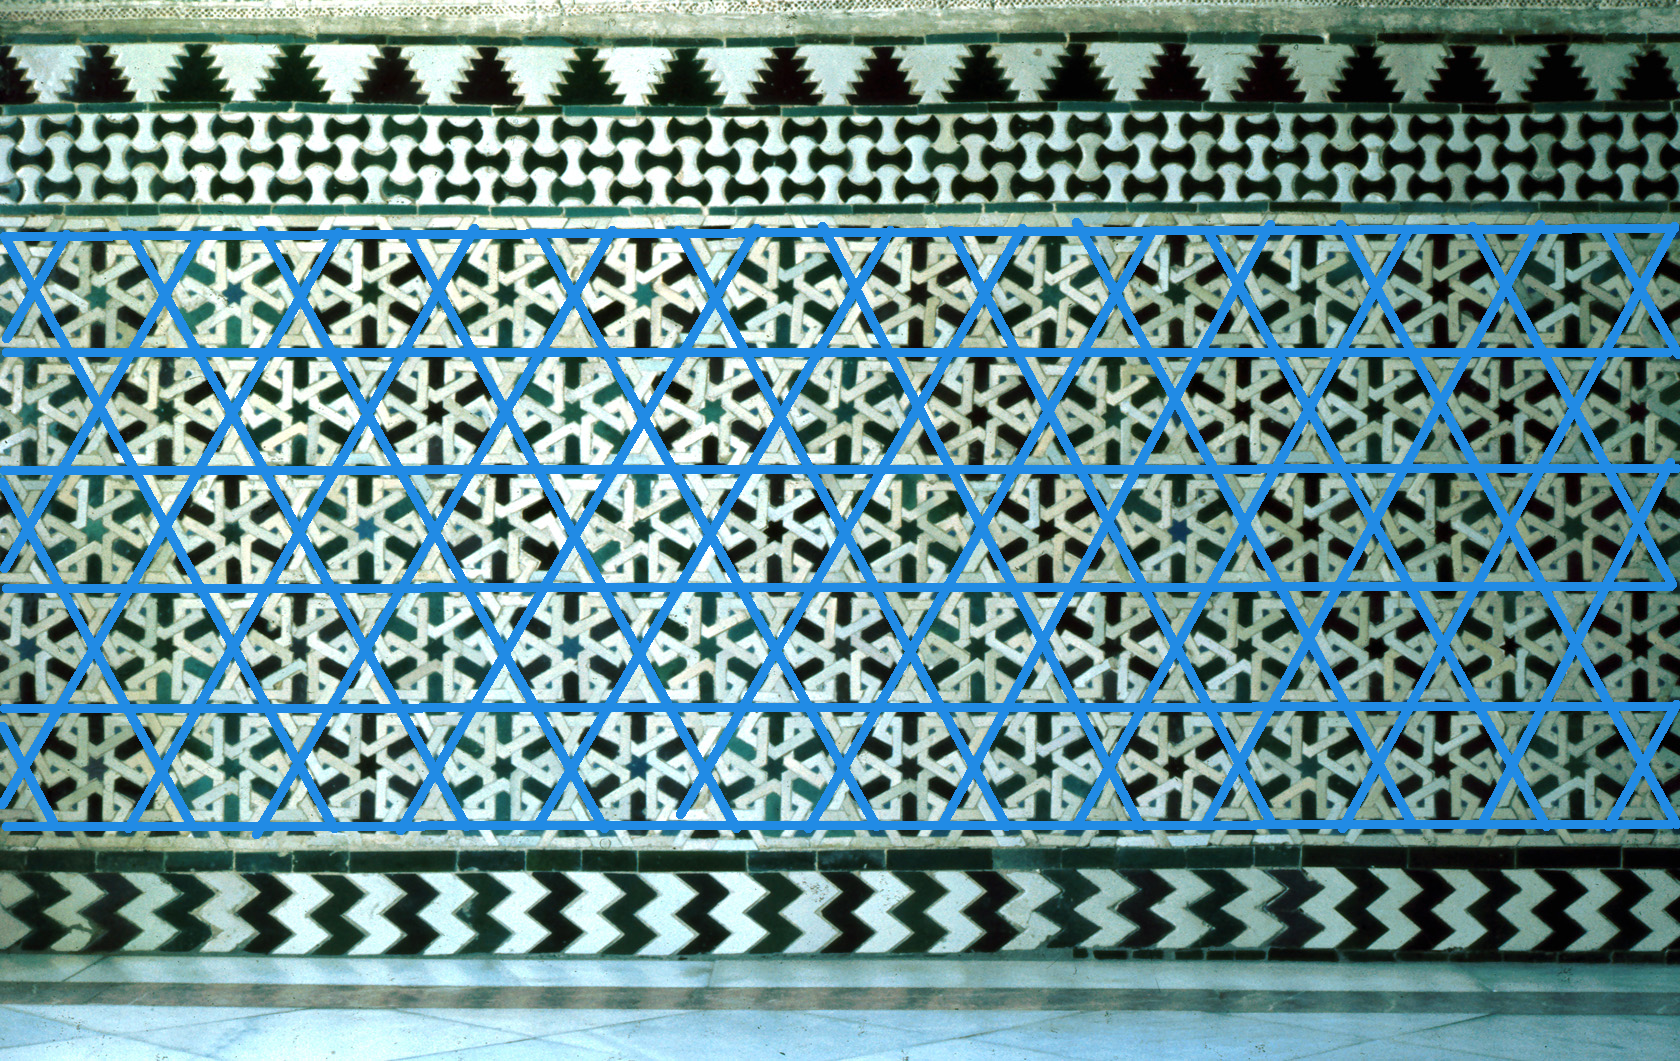
\includegraphics[scale=8]{Alcazar-Kagome.png}}}
          \only<3>{\put(-100,-70){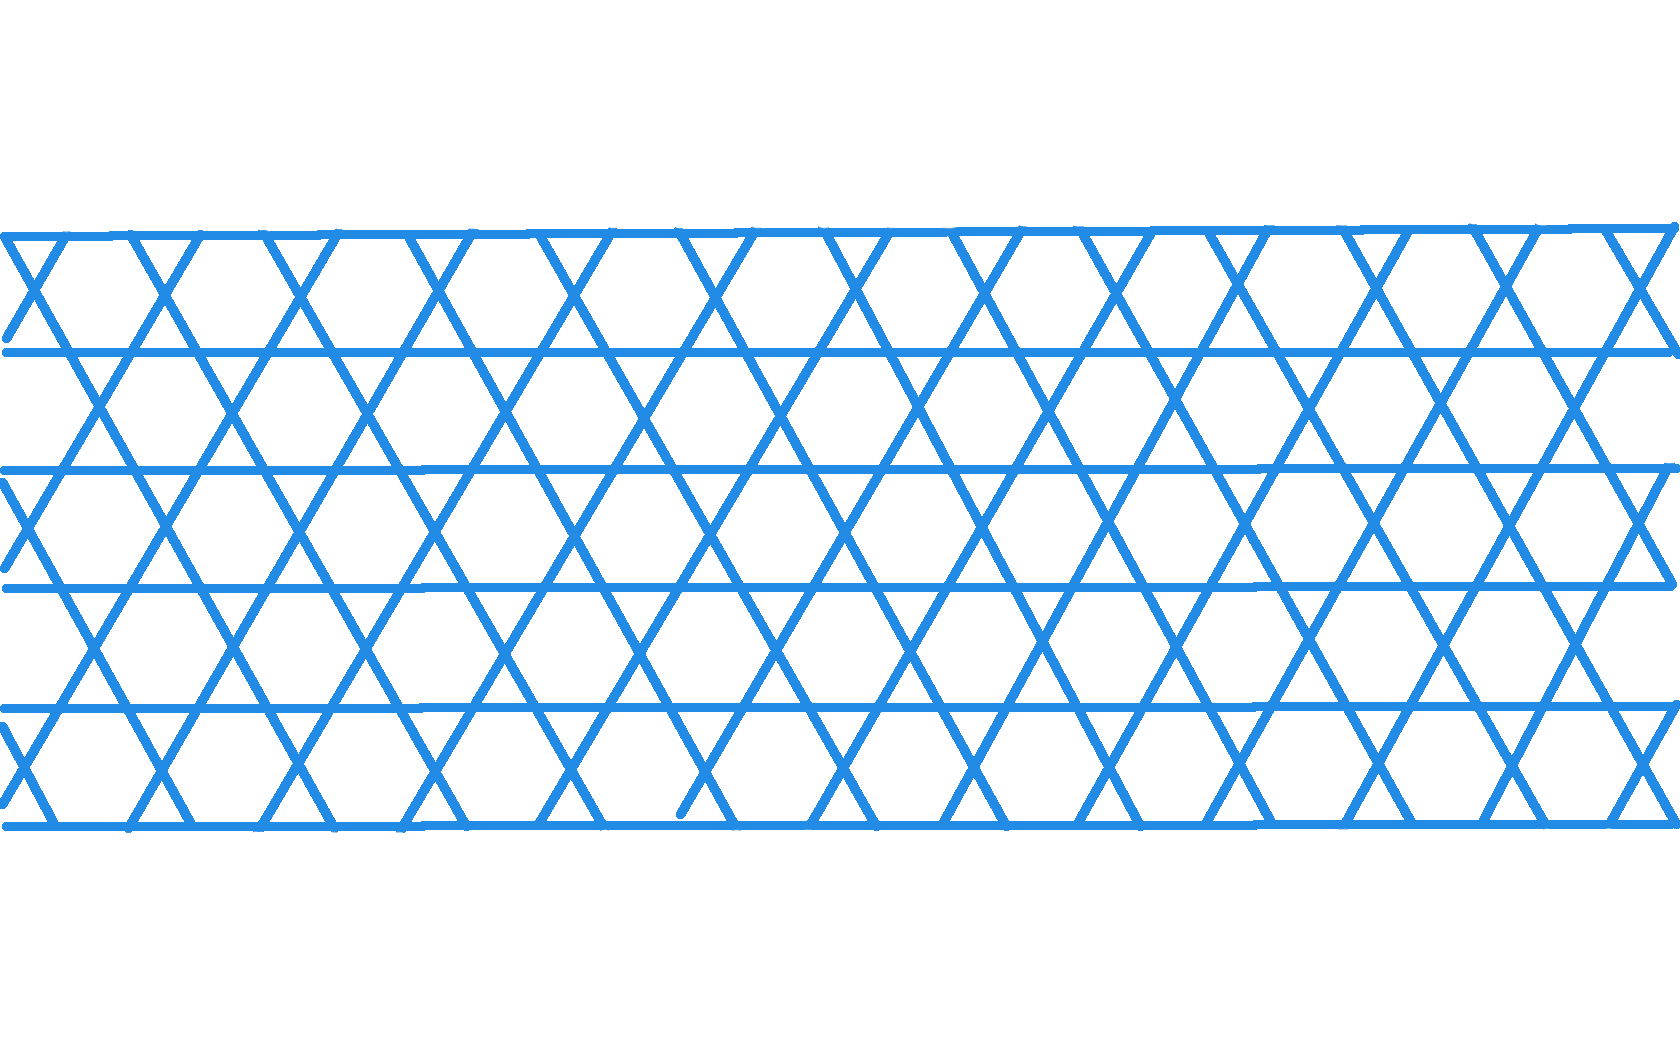
\includegraphics[scale=8]{Kagome.png}}}
          \only<4>{\put(-100,-70){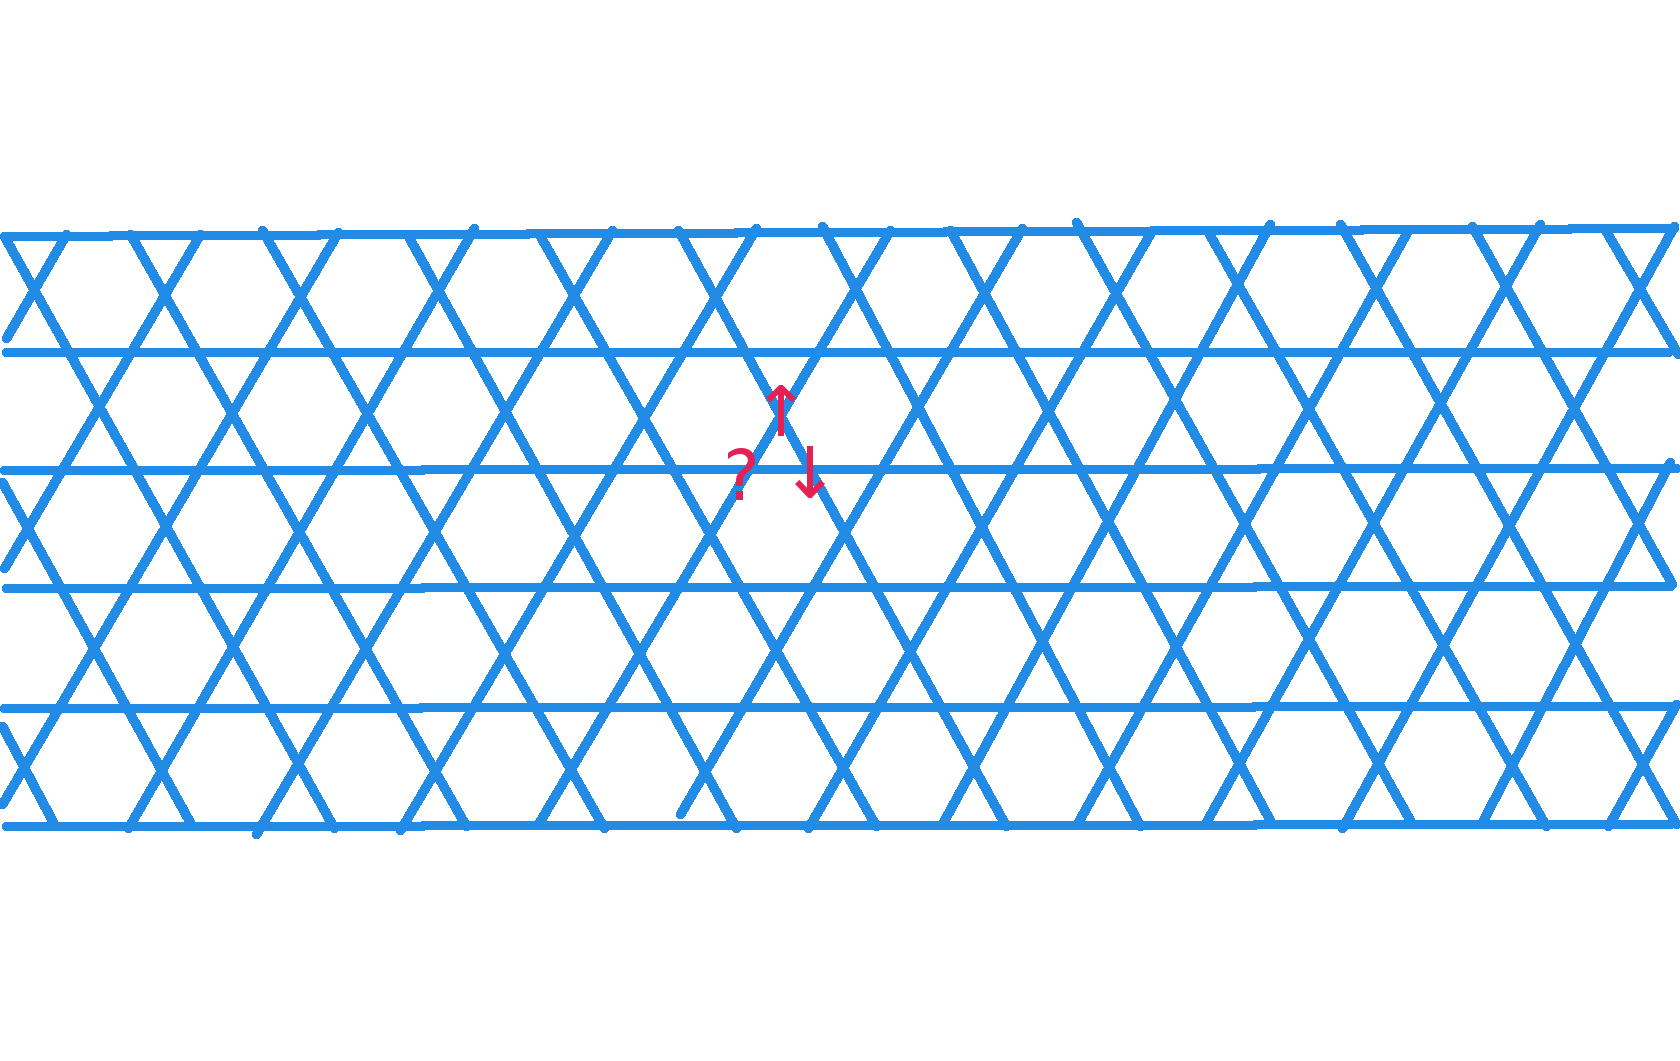
\includegraphics[scale=8]{Kagome-spins.png}}}
          % \only<5>{includegraphics[scale=8]{HAF.png}}
        \end{picture}
      \end{center}
%      \end{overlayarea}

    \end{frame}

    \begin{frame}
      \frametitle{Introduction}
      \begin{itemize}
      \item Goal: study low-energy eigenvectors (low-temperature properties) of
        $H_{AF}$ on subgraphs of the Kagome lattice.
      \item<2-> In the \emph{large spin limit} $S\to +\infty$, one
        should recover the geometry of the classical energy landscape.\footcite{doucot_semiclassical_1998}
      \item<2-> Minimisers of
        \[
          (\S^2)^{|G|} \mapsto \sum_{e\sim f}u_e\cdot u_f
        \]
        form a very complicated set! Not a smooth manifold.
      \end{itemize}
    \end{frame}

\begin{frame}\frametitle{Introduction}
\begin{center}
	\begin{tabular}{|c|c|}
		\spline
	    Classical mechanics & Quantum mechanics\\
		\spline
		Symplectic manifold $M$ & Hilbert Space $H$\\ 
		\spline 
		Function $a\in C^{\infty}(M,\R)$ & Self-adjoint
                                                   operator $A\in L(H)$\\
		\spline
                Hamiltonien flow of $a$ & Flow of $e^{itA/\hbar}$\\
		\spline
		Poisson Bracket & Lie Bracket\\
		\spline
	\end{tabular}\end{center}\vspace{0em}
	\begin{itemize}
	\uncover<2>{\item Quantization : for a given classical
          model, how to construct an associated quantum
          model ?
	
	\item Semiclassics : the quantum model is $\hbar$-dependent. What
          can be said in the $\hbar\to 0$ limit ?}
	\end{itemize}
\end{frame}

\AtBeginSection
{
	\begin{frame}
		\frametitle{Plan}
		\tableofcontents[currentsection]
	\end{frame}
	
}

\section{Toeplitz operators}
\subsection{Toeplitz operators on $\C^n$}
\begin{frame}
  \frametitle{Bargmann spaces}
  \begin{itemize}
  \item Original idea: express Quantum Mechanics directly in phase
    space.\footcite{bargmann_hilbert_1961}
  \uncover<2->{\item The standard $L^2(\R^n)$ is replaced with the \emph{Bargmann
      space}, with parameter $N>0$:
$$B_N=L^2(\C^n)\cap\left\{e^{-\frac N2 |\cdot|^2}f,\,f\text{ is
  holomorphic on $\C^n$}\right\}.$$}\vspace{-2em}
  \uncover<3>{\item This is a closed subspace of $L^2(\C^n)$, with reproducing
    kernel
$$\Pi_N(x,y)=\left(\frac N{\pi}\right)^n\exp\left(-\cfrac N2
  |x-y|^2+iN\Im(x\cdot \overline{y})\right).$$}
  \end{itemize}

\end{frame}

\begin{frame}
  \frametitle{Toeplitz quantization}
  Let $f\in C^{\infty}(\C^n,\C)$ bounded. The Toeplitz operator associated
  with $f$ is the bounded operator
\begin{center}
\begin{array}{rcl}
 		T_N(f):B_N(\C^n)&\mapsto & B_N(\C^n)\\
		u& \mapsto& \uncover<2->{\Pi_N(}fu\uncover<2->{)}.
 		\end{array}
\end{center}

\uncover<3->{If $f$ has polynomial growth then $T_N(f)$ is an unbounded operator
with dense domain.}
\uncover<4>{\begin{itemize}
\item If $f$ is real-valued then $T_N(f)$ is ess. self-adjoint.
\item If moreover $f\geq 0$ then $T_N(f)\geq 0$.
\end{itemize}}
\end{frame}

\begin{frame}
  \frametitle{Composition of Toeplitz operators}
  \begin{itemize}
  \item Recipe: \[T_N(z\mapsto \overline{z}^{\alpha}z^{\beta})=N^{-|\alpha|}\partial^{\alpha}z^{\beta}.\]

\uncover<2->{\item The Toepliz quantization is \emph{anti-Wick}: if $f$ is
  anti-holomorphic and $h$ is holomorphic then
\[T_N(fgh)=T_N(f)T_N(g)T_N(h).\]}
\uncover<3>{\vspace{-1.5em}\item More generally, composition yields a formal series:
\[T_N(f)T_N(g)=T_N\left(fg+N^{-1}C_1(f,g)+N^{-2}C_2(f,g)+\cdots\right).\]

$C_j$ is a bidifferential operator of total order $2j$.}
\end{itemize}
\end{frame}

\begin{frame}
  \frametitle{Toeplitz operators versus $\Psi$DOs}
  \begin{itemize}
  \item The Bargmann transform $\mathcal{B}_N$ conjugates $B_N$ and
    $L^2(\R^n)$.
  \uncover<2->{\item It is related to the FBI
    transform.}
  \uncover<3->{
  \item With $g_N=(N/\pi)^ne^{-N|z|^2}$ one has
    \[
      \mathcal{B}_N^{-1}T_N(f)\mathcal{B}_N=Op_W^{N^{-1}}(f*g_N).
    \]\vspace{-2em}}
\uncover<4->{\item Formal equivalence between Toeplitz and $\Psi$DO
  calculus.}
\uncover<5>{\item Toeplitz quantization is formulated directly in
  phase space, and it is positive.}

  \end{itemize}
\end{frame}

\subsection{Toeplitz operators on compact manifolds}
\begin{frame}
  \frametitle{Hardy spaces and Szeg\H{o} kernel}
  \begin{itemize}
  \item Geometrical setting: compact, complex, symplectic manifold $M$
    under compatibility conditions\footcite{woodhouse_geometric_1997}; complex line bundle $L$ over $M$.
\uncover<2->{\item Quantum space $H_N(M,L)$ of holomorphic sections of
  $L^{\otimes N}$ (holomorphic functions are constant).}
\uncover<3->{\item Szeg\H{o} projector $S_N:L^2(M,L^{\otimes N})\to H_N(M,L).$}
  \end{itemize}
\uncover<4>{The spaces $H_N(M,L)$ are finite-dimensional in that case. The
line bundles $L^{\otimes N}$ correspond to the weights $e^{-\frac N2
  |\cdot|^2}$ in the flat case.}
\end{frame}

\begin{frame}
  \frametitle{Algebra of Toeplitz operators}
  \begin{itemize}
  \item As $N\to +\infty$, the Szeg\H{o} kernel $S_N$ has a full expansion near the
    diagonal, and decays far from it\footcite{charles_berezin-toeplitz_2003,berman_direct_2008}.
  \uncover<2->{\item Indeed $S_N$ can be seen as the $N$-th Fourier mode of a
    Fourier Integral Operator with complex phase; the critical set is
    the diagonal.\footcite{boutet_de_monvel_sur_1975}}
\uncover<3->{\item The dominant term is always $\Pi_N$.}
  \uncover<4>{\item Toeplitz operators form a $C^{*}$-algebra as previously.} 
  \end{itemize}
\end{frame}

\begin{frame}
  \frametitle{An example: the 2D sphere}
  Here $M=\mathbb{S}^2$. In the stereographic projection, $L$
  corresponds to the weight $z\mapsto \frac{1}{1+|z|^2},$ so
  that \begin{align*}H_N(M,L)&\simeq \left\{f\text{ holomorphic in
                               $\C$},\,\int_{\C}\cfrac{|f|^2}{(1+|z|^2)^{N+2}}<\infty\right\}\\
                             &=\C_N[X].\end{align*}
                           \uncover<2->{Expression of the Szeg\H{o}
                             kernel:\[S_N(z,w)=\cfrac{N+1}{\pi}\left(\cfrac{1+z\overline{w}}{\sqrt{(1+|z|^2)(1+|w|^2)}}\right)^N.\]}
\uncover<3>{In the canonical basis $\binom{N}{k}^{-\frac 12}X^k$, the Toeplitz
quantization of the three base coordinates on $\mathbb{S}^2$ are the Spin
matrices with spin $S=\frac {N-1}2$.}
\end{frame}

\section{localisation of ground states}
\subsection{Localisation at the classical minimal set}
\begin{frame}
  \frametitle{Speed of localisation}
  Spectral study of a Toeplitz operator $T_N(f)$: normalised
  eigenvector $u_N$ at smallest eigenvalue (can be degenerate).
  \begin{itemize}
    \item<2->  If $f$ is smooth, the ground state decays
      rapidly in the forbidden region: if $V$ is such that
      $\inf_V(f)>\min_M(f)$, then \[\int_{V}|u_N|^2=O(N^{-\infty}).\]
    \item<3> If $f$ is analytic, the ground state decays exponentially
      fast\footcite{deleporte_toeplitz_2018}: there exists $c>0$ such that
      \[
        \int_{V}|u_N|^2=O(e^{-cN}).
      \]\vspace{-1em}
    \end{itemize}
\uncover<3>{Tool for the analytic case: new analytic microlocal
  methods}
  \end{frame}

\subsection{Subprincipal effects on localisation}
\begin{frame}
  \frametitle{Characteristic value}
  Can one improve the lower bound $f\geq 0\Rightarrow T_N(f)\geq 0$?
  \begin{itemize}
  \item If $q$ is a quadratic form in $\C^n$, the minimal eigenvalue
    of $T_N(q)$ is $N^{-1}\mu(q)$ with $$\mu(q)=N^{-1}(Tr^+(q)+\frac
    12 \tr(q)).$$
  \uncover<2>{\item Here, up to a
    symplectomorphism, $$q=\sum_{i=1}^{r}\lambda_i(q_i^2+p_i^2)+\sum_{i=r+1}^{r+r'}p_i^2,$$
    so $$Tr^+(q)=\sum_{i=1}^r\lambda_i.$$
}

\end{itemize}
\end{frame}

\begin{frame}
  \frametitle{Melin estimate and ground state concentratoin}
  \begin{minipage}[l]{0.3\linewidth}\vspace{1em}\begin{center}
    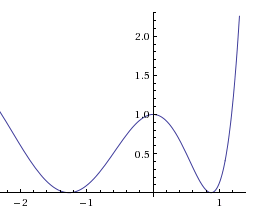
\includegraphics[width=0.8\linewidth]{wells.png}\\
    \uncover<2>{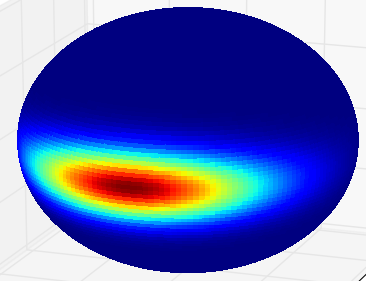
\includegraphics[width=0.7\linewidth]{35.png}}
  \end{center}
\end{minipage}%
  \begin{minipage}[r]{0.65\linewidth}
    \begin{itemize}
    \item If $f$ is minimal at several non-degenerate points, ground
      states only concentrates at the wells which are ``minimal'' for
      the Melin value.\footcite{deleporte_low-energy_2016-1}\vspace{1em}
    \item<2-> Arbitrary $f$: same result.\footcite{deleporte_low-energy_2017}
    \end{itemize}
  \end{minipage}
\end{frame}



\begin{frame}
  \frametitle{Two particular cases}
  \begin{itemize}
  \item ``Miniwells''\footcite{helffer_puits_1986}: $\mu$ is only minimal at one point $x_0$ near which $\{f=0\}$ is
    an isotropic submanifold, and the minimum is non-degenerate,
    expansions for the smallest eigenvalue and the associated
    eigenvector.\footcite{deleporte_low-energy_2017}
  \item ``Crossing case'' as in the example:
    \[
      f(q_1,q_2,p_1,p_2)=p_1^2+p_2^2+q_1^2q_2^2.
      \]
    Same results.\footcite{deleporte_low-energy_2017}
  \end{itemize}
  Method of proof: symplectic normal forms (new, even for miniwells!)
\end{frame}

\subsection{Future work}
\begin{frame}
  \frametitle{Perspectives}
    \begin{itemize}
    \item Low-energy time evolution
    \item Large dimension (large number of sites)
    \end{itemize}
  \end{frame}

  \begin{frame}
    \frametitle{Publications}
    \printbibliography[keyword=Deleporte,heading=none]
  \end{frame}

  \begin{frame}[allowframebreaks]
    \frametitle{Citations}
    \printbibliography[notkeyword=Deleporte,heading=none]
  \end{frame}
\end{document}
%%% Local Variables:
%%% mode: latex
%%% TeX-master: t
%%% End:
